\documentclass[../../main]{subfiles}

\renewcommand\thesection{\arabic{section}}


\begin{document}

\section{Ways of Asking Questions} \label{sec:}

There are several ways to implement an algorithm. One
way is to use an \emph{if-else} to parse through the data available.
Figure \ref{fig:differentWaysOfModeling} (a) depicts such a
method. Like wise, one be able to transform the inputs
directly into output\footnote{Given that we know the coefficients of
transforming matrix.}. Figure \ref{fig:differentWaysOfModeling} (b)
shows such a transforming matrix\footnote{They need not be 2 dimensional
but could be N dimensional.}.


\begin{center}

    \setlength{\arraycolsep}{0.15cm}
    % \renewcommand\arraystretch{1.75}


    \begin{tabularx} {\textwidth} {
            >{\centering \arraybackslash}X
            >{\centering \arraybackslash}X
        }

        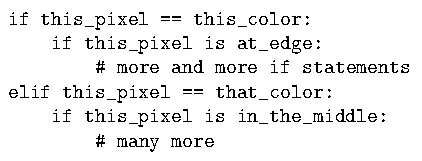
\includegraphics [width = 0.5\textwidth] {pics/if_else_code.pdf}

        &

            $\begin{pNiceMatrix}
                c_{11} & c_{12} & c_{13} & c_{14} & \cdots & c_{1n} \\
                c_{21} & c_{22} & c_{23} & c_{24} & \cdots & c_{2n} \\
                c_{31} & c_{32} & c_{33} & c_{34} & \cdots & c_{3n} \\
                c_{41} & c_{42} & c_{43} & c_{44} & \cdots & c_{4n} \\
                \vdots & \vdots & \vdots & \vdots & \ddots & \vdots\\
                c_{m1} & c_{m2} & c_{m3} & c_{m4} & \cdots & c_{mn} \\
            \end{pNiceMatrix}$

        \\
        \vspace{0.35cm}
        (a)
        &
        \vspace{0.35cm}
        (b)
        \\

        % \bottomrule
        \multicolumn{2}{c}{
            \begin{minipage} {\textwidth}
                \vspace{0.25cm}
                \captionof{figure}{Two ways to model our questions.}
                \label{fig:differentWaysOfModeling}
            \end{minipage}
        }


    \end{tabularx}

\end{center}

In some sense, a matrix transform is much more of a compact version of the \emph{if-else}
statement. Matrix operations are parallelizable, therefore operations like these can
be accelerated using dedicated hardware like GPUs.

% \begin{minipage} {0.425\paperwidth}
%     \centering
% \end{minipage}

\end{document}
